\documentclass{quicknotes}

\usepackage{amsmath}  % Provides \align
\usepackage{graphicx} % Provides \includegraphics
\usepackage{setspace} % Provides \doublespacing
\usepackage[square,numbers]{natbib} % Don't change this. See \citea{} in shortcuts.tex
\usepackage{subcaption} % subfigures
\usepackage{amssymb}  % Provides \because
\usepackage{amsthm} % Enhanced theorem, definition, proof environments from the AMS
\usepackage{booktabs}   % Fancy tables. \toprule, \midrule, \bottomrule commands
% \usepackage{footnote} % Provides \footnote
\usepackage{lipsum}  % Provides \lipsum[n] for filler text

% hyperref: So I can jump around in the PDF
\usepackage[pdftex,hyperfootnotes=false,pdfpagelabels]{hyperref}
\hypersetup{
    colorlinks=true, linktocpage=true, pdfstartpage=1, pdfstartview={FitH},
    breaklinks=true, pdfpagemode=UseNone, pageanchor=true, pdfpagemode=UseOutlines,
    plainpages=false, bookmarksnumbered, bookmarksopen=true, bookmarksopenlevel=1,
    hypertexnames=true, pdfhighlight=/O,%nesting=true,%frenchlinks,
    urlcolor=webbrown, linkcolor=RoyalBlue, citecolor=webgreen, %pagecolor=RoyalBlue,
    pdftitle={Example document for quicknotes LaTeX class},
    pdfauthor={Author Name},
    pdfsubject={QuickNotes Latex template},
    pdfkeywords={quicknotes, latex, template},
    pdfcreator={pdfLaTeX},
    pdfproducer={LaTeX with hyperref and quicknotes}
}
\usepackage[all]{hypcap} % Makes sure that link to figure/table shows the figure/table instead of the caption

% 'code' is shorter than verbatim
\usepackage{fancyvrb}
\DefineShortVerb{\|}
% \VerbatimFootnotes   % Causes stack error. See https://tex.stackexchange.com/questions/203/how-to-obtain-verbatim-text-in-a-footnote
\DefineVerbatimEnvironment{code}{Verbatim}
{
    frame=single,
    framesep=0.25em,
    xleftmargin=1em,
    xrightmargin=1em,
    samepage=true,
    fontsize=\footnotesize
}

\begin{document}
\title{Example document for quicknotes \LaTeX{} class}
\author{Author Name\thanks{Some email address}}
\date{\today}
\maketitle
\begin{abstract}
This is a short example of how to use the \texttt{quicknotes} class. Please see the PDF for a
demo of how the final result may look like. This theme is a quick version of the
\href{https://github.com/ankur-gupta/uwcbethesis}{uwcbethesis} theme.
\end{abstract}

\section{Section 1}
The Einstein field equations~\cite{einstein1916foundation} can be displayed nicely as follows.
\begin{equation}
R_{\mu\nu} - \frac{1}{2} R g_{\mu\nu} + \Lambda g_{\mu\nu} = \frac{8 \pi G}{c^4} T_{\mu\nu}
\label{eqn:efe}
\end{equation}
In comparison, Newton's law of gravitation is written as follows:
\begin{equation}
F = -G\frac{m_1 m_2}   {r^2}
\end{equation}
in which, $F$ is the attractive force between two point objects that have masses $m_1$ and $m_2$
and are separated by a scalar distance of $r$.

\subsection{Section 1.1}
You can refer to Eq~\ref{eqn:efe} easily. A random variable $X\sim \text{Bernoulli}(p)$ is
Bernoulli distributed when it follows the distribution:
\begin{align}
P(X = x) = \begin{cases}
px + (1-p)(1-x) & x \in \{0, 1\} \\
0 & \text{otherwise}
\end{cases} \label{eqn:bernoulli}
\end{align}

\subsection{Section 1.2}
Table \ref{tab:famousswords} shows a dummy table, copied from
\href{https://github.com/ankur-gupta/uwcbethesis}{uwcbethesis}.

\begin{table}
\caption{Famous Swords}
\label{tab:famousswords}
\centering
\begin{tabular}{lll}
\toprule
Sword Name & Intended Swordsman & Story\\
\midrule
Excalibur & King Arthur & Arthurian legend \\
Ice & Eddard Stark & A Song of Fire and Ice \\
And\'{u}ril & Aragorn & Lord of the rings \\
\bottomrule
\end{tabular}
\end{table}

\section{Section 2}
Multiplicative form of the Bernoulli distribution is provided in Eq~\ref{eqn:bernoulli}.

\subsection{Section 2.1}
You can cite references too like this~\cite{einstein1916foundation}.
A footnote looks like this\footnote{This is a footnote.}.
Verbatim code can be written like this:
\begin{code}
~/texmf/bibtex/bib/
\end{code}

\section{Section 2.3}
Figure~\ref{fig:cat} provides an obligatory cat picture.

\begin{figure}
\centering
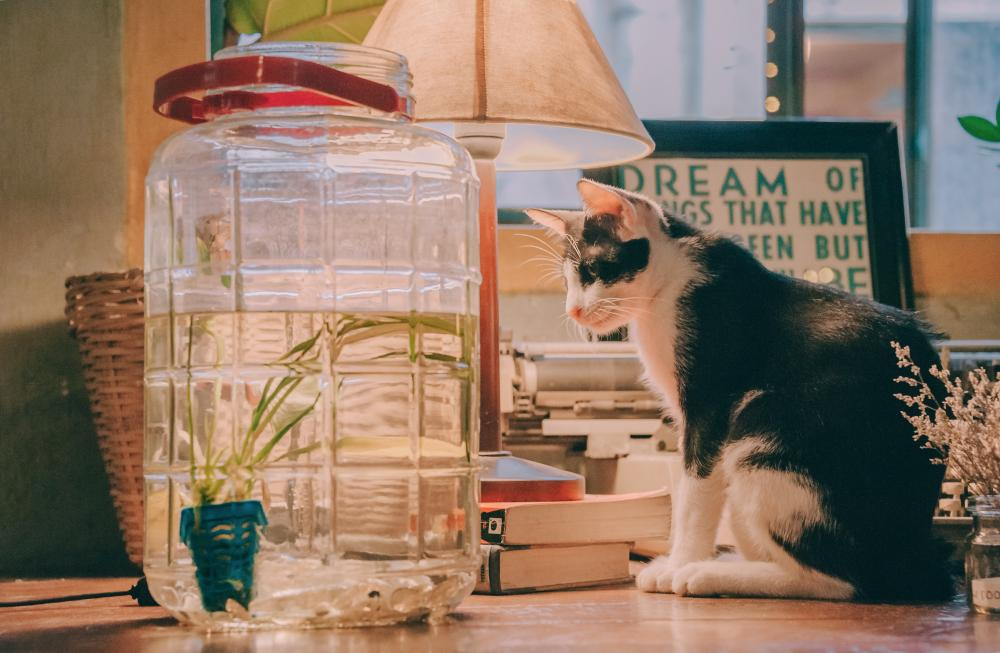
\includegraphics[width=0.5\textwidth]{cat.jpg}
\caption{Curious cat (thanks to Pexels!)}
\label{fig:cat}
\end{figure}

\bibliographystyle{acm}
\bibliography{citations}

\end{document}